\documentclass[tikz]{standalone}
\standaloneconfig{border=0.3cm}
\usepackage[utf8]{inputenc}
\usepackage{nicefrac}

\usetikzlibrary{positioning}
\usetikzlibrary{shapes.geometric}
\tikzstyle{blok} = [
  rectangle, minimum width=1.0cm, minimum height=0.75cm, thin, draw=black,
]

\tikzstyle{kopje}=[align=left, anchor=west, text width=10cm, font={\bfseries}]
\tikzstyle{subkopje}=[align=left, anchor=west, text width=1cm, font={\footnotesize}]
\tikzstyle{gen}=[align=left, anchor=west, text width=3.5cm, font={\footnotesize \itshape}]
\tikzstyle{int}=[align=center, anchor=west, font={\footnotesize \itshape}]
\tikzstyle{particle}=[align=center, font={\itshape \LARGE}]
\tikzstyle{pname}=[align=center, font={\scriptsize}]

\begin{document}

\tikzset{arrow/.style={-stealth, thin, draw=black}}
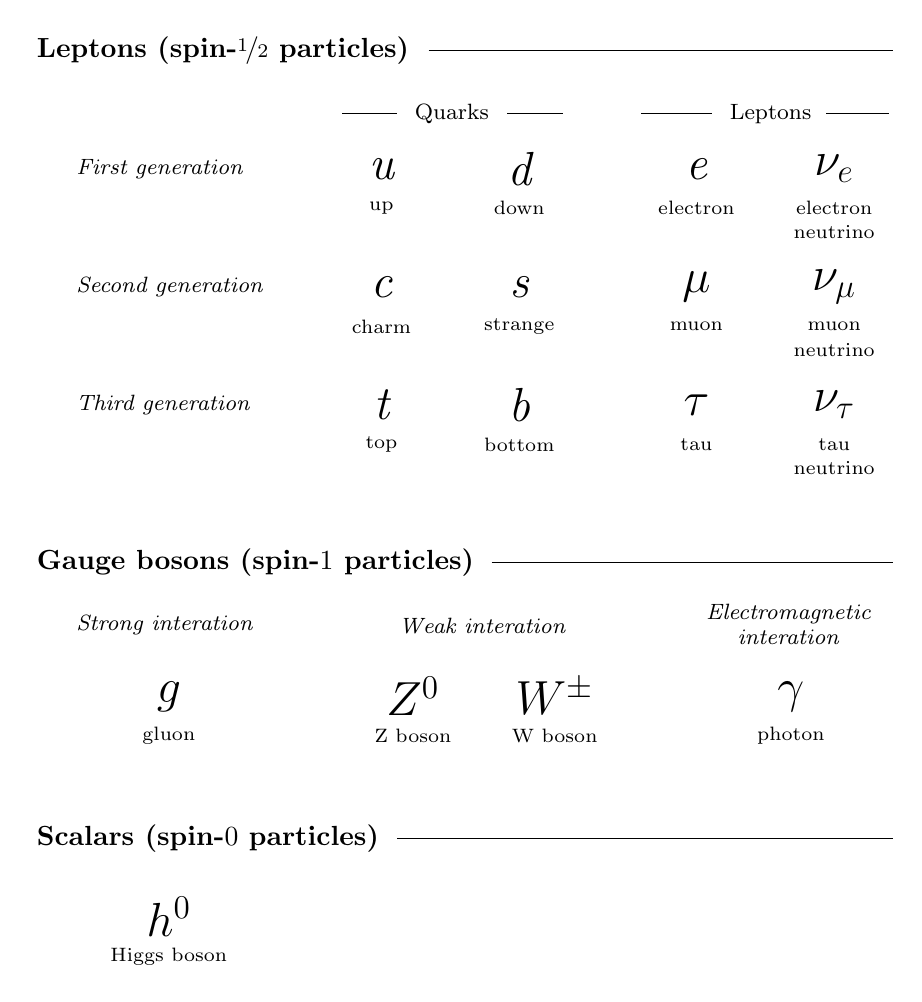
\begin{tikzpicture}

\node[kopje]     (fermions) at (0.0, 10.0)  {Leptons (spin-$\nicefrac{1}{2}$ particles)};

\node[gen]       (gen1)     at (0.5,   8.5) {First generation};
\draw (5.1, 10.0) -- (11.0, 10.0);

\node[subkopje]  (quarks)   at (4.8,   9.2) {Quarks};
\node[subkopje]  (quarks)   at (8.8,   9.2) {Leptons};
\draw (4.0, 9.2) -- (4.7, 9.2);
\draw (6.1, 9.2) -- (6.8, 9.2);
\draw (7.8, 9.2) -- (8.7, 9.2);
\draw (10.15, 9.2) -- (10.95, 9.2);

\node[particle]  (u)        at (4.5,   8.5) {u};
\node[particle]  (d)        at (6.25,  8.5) {d};
\node[particle]  (e)        at (8.5,   8.5) {e};
\node[particle]  (ve)       at (10.25, 8.5) {$\nu_e$};
\node[pname]     (uname)    at (4.5,   8.0) {up};
\node[pname]     (dname)    at (6.25,  8.0) {down};
\node[pname]     (ename)    at (8.5,   8.0) {electron};
\node[pname]     (vename1)  at (10.25, 8.0) {electron};
\node[pname]     (vename2)  at (10.25, 7.7) {neutrino};

\node[gen]       (gen2)     at (0.5,   7.0) {Second generation};
\node[particle]  (c)        at (4.5,   7.0) {c};
\node[particle]  (s)        at (6.25,  7.0) {s};
\node[particle]  (mu)       at (8.5,   7.0) {$\mu$};
\node[particle]  (vmu)      at (10.25, 7.0) {$\nu_\mu$};
\node[pname]     (cname)    at (4.5,   6.5) {charm};
\node[pname]     (sname)    at (6.25,  6.5) {strange};
\node[pname]     (muname)   at (8.5,   6.5) {muon};
\node[pname]     (vmuname1) at (10.25, 6.5) {muon};
\node[pname]     (vmuname2) at (10.25, 6.2) {neutrino};

\node[gen]       (gen3)     at (0.5,   5.5) {Third generation};
\node[particle]  (t)        at (4.5,   5.5) {t};
\node[particle]  (b)        at (6.25,  5.5) {b};
\node[particle]  (tau)      at (8.5,   5.5) {$\tau$};
\node[particle]  (vtau)     at (10.25, 5.5) {$\nu_\tau$};
\node[pname]     (tname)    at (4.5,   5.0) {top};
\node[pname]     (bname)    at (6.25,  5.0) {bottom};
\node[pname]     (tauname)  at (8.5,   5.0) {tau};
\node[pname]     (vtauname1) at (10.25, 5.0) {tau};
\node[pname]     (vtauname2) at (10.25, 4.7) {neutrino};

\node[kopje]     (bosons)   at (0.0, 3.5) {Gauge bosons (spin-$1$ particles)};
\draw (5.9, 3.5) -- (11.0, 3.5);

\node[int]       (strong)   at (0.5, 2.7) {Strong interation};
\node[particle]  (g)        at (1.8, 1.8) {$g$};
\node[pname]     (gname)    at (1.8, 1.3) {gluon};

\node[int]       (em)       at (4.6, 2.7) {Weak interation};
\node[particle]  (z)        at (4.9, 1.8) {$Z^0$};
\node[pname]     (zname)    at (4.9, 1.3) {Z boson};
\node[particle]  (w)        at (6.7, 1.8) {$W^\pm$};
\node[pname]     (wname)    at (6.7, 1.3) {W boson};

\node[int]       (em1)      at (8.5, 2.85)  {Electromagnetic};
\node[int]       (em2)      at (8.9, 2.55)  {interation};
\node[particle]  (photon)   at (9.7, 1.8)   {$\gamma$};
\node[pname]     (photname) at (9.7, 1.3)   {photon};


\node[kopje]     (scalars)  at (0.0, 0.0)  {Scalars (spin-$0$ particles)};
\draw (4.7, 0.0) -- (11.0, 0.0);

\node[particle]  (h)        at (1.8, -1.0) {$h^0$};
\node[pname]     (hname)    at (1.8, -1.5) {Higgs boson};

\end{tikzpicture}

\end{document}
